\chapter{Teszteredmények} \label{Testing}
Ebben a fejezetben a tesztelése menete, a tesztelés által elért eredmények kerülnek bemutatásra.
Mivel esetemben egy meglévő szoftver rendszer továbbfejlesztéséről beszélhetünk, ezért az új funkciók letesztelésén kívül fontos az eddigi funkcionalitás újratesztelése is.
Éppen ezért a tesztesetek alapvetően három részre bonthatóak:
\begin{itemize}
\item A determinisztikus throughput maximalizáló tesztelése
\item A sztochasztikus alapesetek tesztelése
\item A sztochasztikus multiproduct esetek tesztelése
\end{itemize}
A teszteléshez használt input fájlok tartalma, nevezetesen a termékekre, illetve a forgatókönyvekre vonatkozó paraméterek random szám generátorral készültek adott tartományokon belül.
A tesztkonfigurácó leírása:
\begin{itemize}
\item Windows 7 operációs rendszer 
\item Qt 5.11.2, Microsoft Visual C++ Compiler 15.0, Boost Libraries 1.68.0
\item Intel i5 3570K 3,8 Ghz processzor
\item 8 GB RAM
\end{itemize}
\section{A determinisztikus throughput maximalizáló tesztelése}
A determinisztikus throughput maximalizáló teszteléséhez használt teszt fájlok a CD melléklet  \fileName{Tesztelés/Tesztfájlok/Determinisztikus} mappájában találhatóak, míg a teszteredményeket rögzítő \fileName{DeterministicTestResults.ods} fájl a CD melléklet \fileName{Tesztelés/Teszteredmények} mappájában található.
A determinisztikus teszt fájlokban található termékek profit értékei véletlenszerűen választott számok, a többi adat pedig a \fileName{multipurpose.ods} fájlból került átmásolásra.
A \ref{deterministic_test}. ábrán látható egy példa egy determinisztikus teszt fájlra.
\begin{figure}[H]
\begin{center}
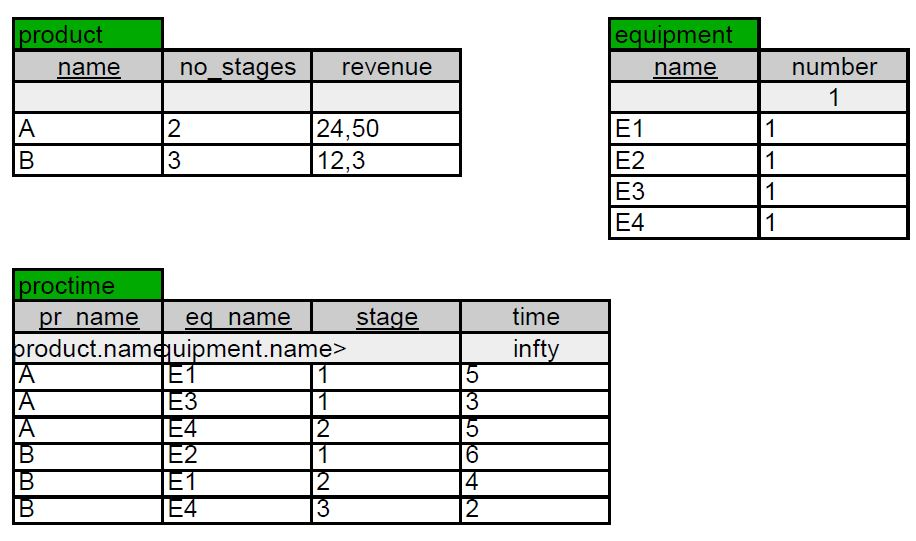
\includegraphics[scale=0.5]{deterministicTest}
\caption{Példa egy determinisztikus teszt fájlra}
\label{deterministic_test}
\end{center}
\end{figure}
Ezen fájlt felhasználva például a determinisztikus throughput maximalizáló 15 óra időhorizont érték mellett 61.3 profit egységet adott eredményül a következő gyártott mennyiségek mellett: $2A+1B$.
Jól látható, hogy az eredmény helyes, hiszen $2 \cdot 24.5 +12,3=61.3$.
Ezenfelül a solver master git branchén található verziót futtatva (melyhez a dolgozat írásakor még nem került hozzáadásra a munkám) szintén megegyező eredményt kapunk, mind a profit értékeket, mind a kimeneti ütemterveket figyelembe véve, valamint a futási időkben sem figyelhető meg számottevő változás.
A \fileName{DeterministicTestResults.ods} fájl adatait figyelembe véve kijelenthető tehát, hogy a determinisztikus throughput maximalizáló továbbra is hibátlanul működik.     
\section{A sztochasztikus alapesetek tesztelése}
A sztochasztikus throughput maximalizáló alapeseteinek teszteléséhez használt teszt fájlok a CD melléklet  \fileName{Tesztelés/Tesztfájlok/Sztochasztikus} mappájában találhatóak, míg a teszteredményeket rögzítő \fileName{StochasticTestResults.ods} fájl a CD melléklet \fileName{Tesztelés/Teszteredmények} mappájában található.
A sztochasztikus teszt fájlokban található, a termékekre, illetve a forgatókönyvekre vonatkozó paraméterek (batch méretek, kereslet, termék ára, stb.) random szám generátorral lettek előállítva.
A \ref{stochastic_test} ábra szemlélteti a \fileName{StochasticTestResults.ods}. fájl tartalmát.
\begin{figure}[H]
\begin{center}
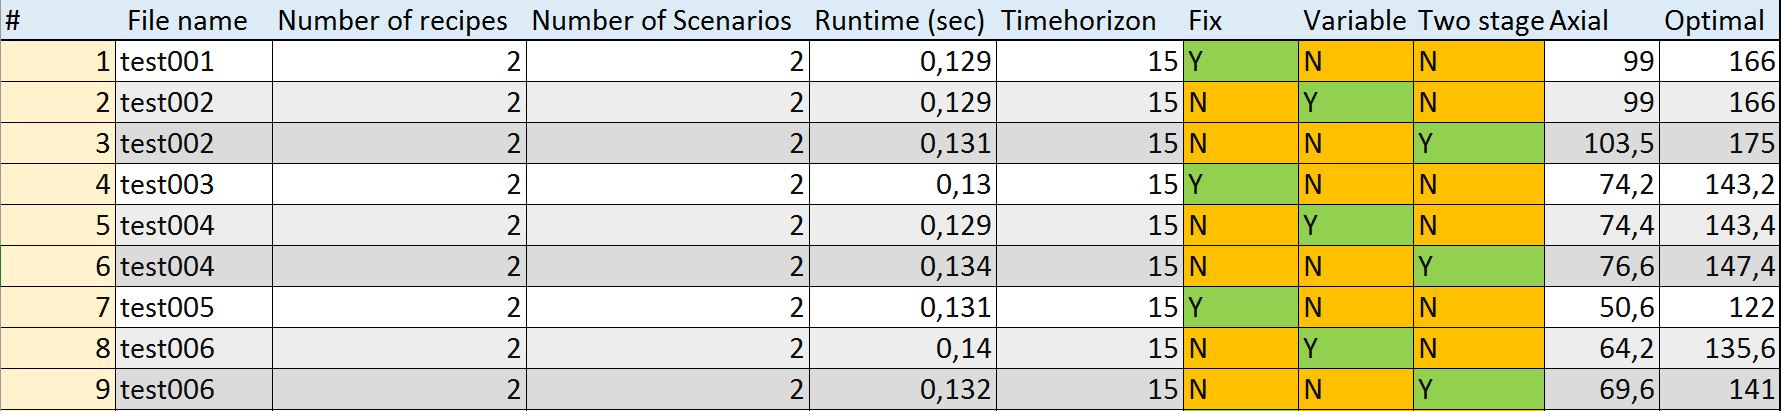
\includegraphics[scale=0.325]{stochasticTest}
\caption{Részlet a \textit{StochasticTestResults.ods} fájlból}
\label{stochastic_test}
\end{center}
\end{figure}
 Az ábra alapján látható, hogy egy teszteset teszteléséhez két különböző fájlra van szükség: egyre a kötött batch méretű esethez, valamint egy másikra a változó batch méretű, illetve a kétlépcsős esethez (hiszen utóbbi bekapcsolásához csupán egy parancssori kapcsolóra van szükség).
Az egy tesztesethez használt fájlokban (Pl. test001 és teszt002) található random generált paraméterek megegyeznek, ezek csupán a batch méretekben térnek el, oly módon, hogy a kötött batch méretű esetben generált számok (Pl. test001 fájl esetén $s_A=8, s_B=10$) a változó batch méretű fájlban a batch méretek alsó, vagy felső korlátait reprezentálják (azaz $s_p^{min}$, vagy $s_p^{max}$ értékének fognak megfelelni), a másik korlátot szintén véletlenszerűen választjuk ki ezekben az esetekben. (Pl. test002 fájl esetén $s_A^{max}=8, s_B^{max}=10$ értékek kerültek beállításra, $s_A^{min}=5, s_B^{min}=7$ értékek lettek generálva.)
Ezen módszert használva felfedhetőek a különböző módok esetleges hibái, könnyen belátható ugyanis, hogy helyes működés esetén a változó batch méretű optimális eredménynek legalább meg kell egyeznie, vagy jobbnak kell lennie a kötött batch méretű várható profit értéknél, hiszen ha a kötött batch méretek a változó batch méretek alsó, vagy felső határát reprezentálják, valamint a solver szabadon választhatja ki $x_p(b_p)$ értéket a $[s_p^{min}\cdot b_p,s_p^{max}\cdot b_p]$ tartományból, az eredmény legrosszabb esetben is a tartomány azon legszélső értéke lesz, amely egyenlő a kötött batch méret esetén számolt $s_p(b_p)$ értékkel.
Hasonló reláció elmondható a változó batch méretű, és a két lépcsős esetek profit értékeire is, hiszen míg a előbbi esetén azonos batch méret kerül beállításra minden forgatókönyv esetén, addig az utóbbi esetben forgatókönyvenként választható meg az ideális batch méret az adott tartományból, tovább növelve esetlegesen a várható profit értékét a változó batch méretű esethez képest, de nem rontva azt a legrosszabb esetben sem.
A tesztesetek között a különböző recept és forgatókönyv darabszámokat tartalmazó eseteken kívül megtalálható néhány speciális eset is:
\begin{itemize}
\item Abban az esetben például, ha a kötött batch méret a változó batch méretű, illetve a két lépcsős esetben a batch méret alsó és a felső korlátja is egyben (test033 és test034), mindhárom várható profit értéknek meg kell egyeznie.
\item Abban az esetben, ha csak egy darab forgatókönyv létezik (test035 és test036), a változó batch méretű eredmény és a két lépcsős eredmény megegyező kell legyen.
\end{itemize}
\begin{figure}[hbtp]
\begin{center}
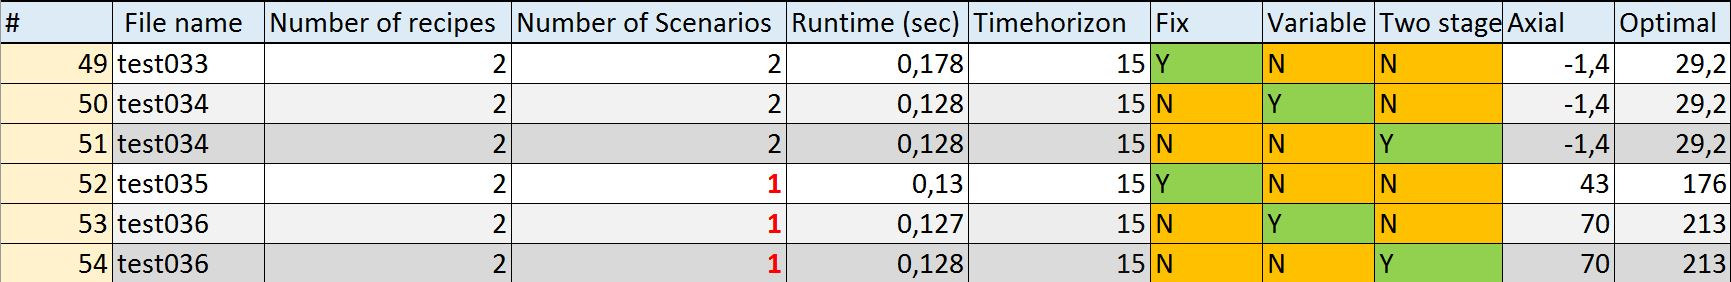
\includegraphics[scale=0.34]{specialTests}
\caption{A speciális teszt esetek eredményei.}
\label{special_tests}
\end{center}
\end{figure} 
A teszteredmények, ahogyan az \ref{stochastic_test}. ábrán, valamint bővebben a \fileName{StochasticTestResults.ods} fájlban is látható alátámasztják a fent leírtakat, tehát a sztochasztikus throughput maximalizáló ilyen szempontból jól működik az alapeseteken, továbbá manuálisan kiszámítva az input fájlokban található paraméterek alapján a várható profit értékét egy találomra választott teszt esetre a \ref{FixBatchSize}. pontban ismertetettek alapján, alátámasztást nyer azon várható profit értékek helyessége is.
\pagebreak
\section{A sztochasztikus multiproduct receptek tesztelése}
A sztochasztikus throughput maximalizáló multiproduct receptekkel való teszteléséhez használt teszt fájlok a CD melléklet  \fileName{Tesztelés/Tesztfájlok/Sztochasztikus\_Multiproduct} mappájában találhatóak, míg a teszteredményeket rögzítő \fileName{StochasticMultiproductTestResults.ods} fájl a CD melléklet \fileName{Tesztelés/Teszteredmények} mappájában található.
Mivel a multiproduct esetek lényegében a sztochasztikus alapesetek speciális változatai, ezért a tesztelés hasonlóképpen zajlik, mint az előző pontban leírtak.
A receptek, termékek, valamint a forgatókönyvek megfelelő adatai véletlenszerűen kerültek kiválasztásra, a tesztesetek lényegében hasonlóak az előző pontban ismertetettekhez, különös figyelmet szentelve az előzőekben már ismertetett speciális esetekre.
A teszteredményeket tartalmazó \fileName{StochasticMultiproductTestResults.ods} fájl felépítése hasonló a \ref{stochastic_test}. ábrán látottakhoz, azzal a bővítéssel, hogy egy plusz oszlop került felvételre a termékek számának dokumentálására.
\begin{figure}[H]
\begin{center}
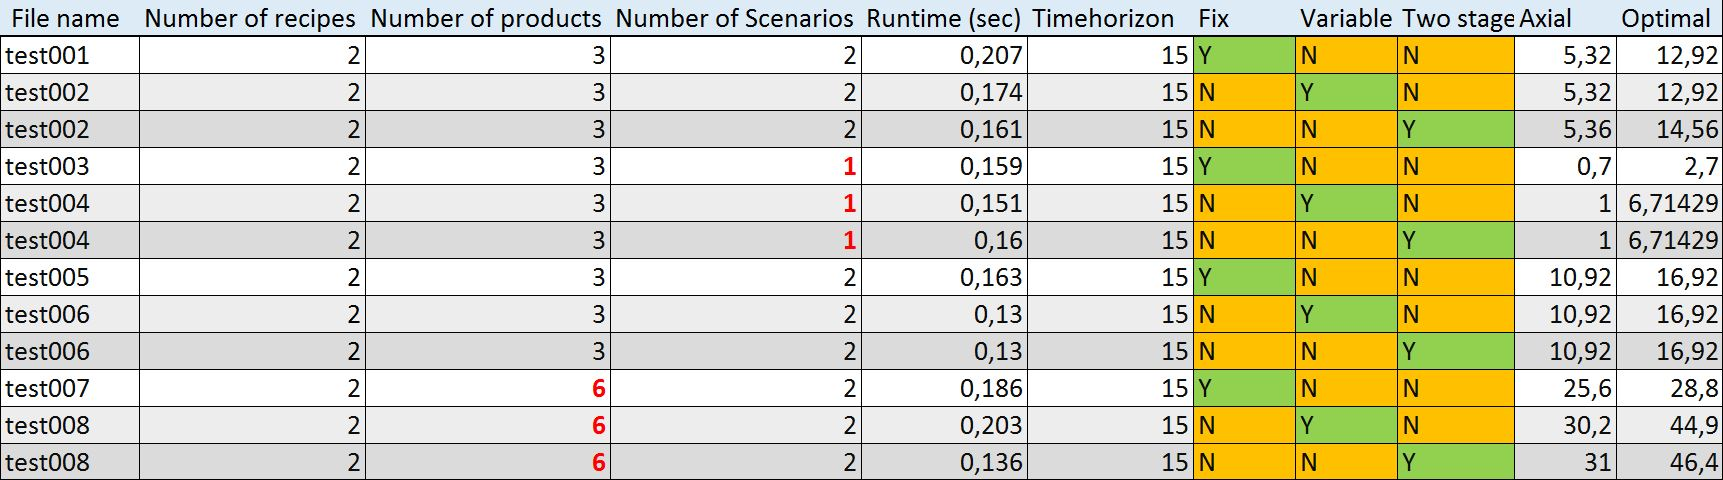
\includegraphics[scale=0.345]{multiproductTests}
\caption{Részlet a \textit{StochasticMultiproductTestResults.ods} fájlból}
\label{multiproduct_test}
\end{center}
\end{figure}
A teszteredmények alátámasztják, hogy a sztochasztikus throughput maximalizáló megfelelően működik az alapesetekhez tartozó inputfájlokkal, illetve multiproduct receptekhez tartozóakkal egyaránt.